\documentclass{beamer}
\usepackage{beamerthemesplit}
\usepackage{booktabs}
\usepackage{graphicx}
\usepackage{transparent}
\usepackage{bbold}
\usepackage[italian]{babel}
\usepackage[utf8x]{inputenc}
\usepackage{listings}
\usepackage{tikz}
\usetikzlibrary{fit, shapes, arrows, patterns, matrix}
\usepackage{amsmath,amsfonts,amssymb}
\usepackage{pgfplots}
\usepackage{scalefnt}
\usepackage{color}
\usepackage{xcolor}
\usepackage{multicol}
\usepackage{bm}

\title[mRMR]{mRMR - features selection method}
\institute{
\begin{small}
Corso di Laurea in Informatica Magistrale
\end{small}}
\author{\textbf{Simone Rutigliano}}
\date{\tiny{\today}}

\usebackgroundtemplate{
%    \transparent{0.12}{
     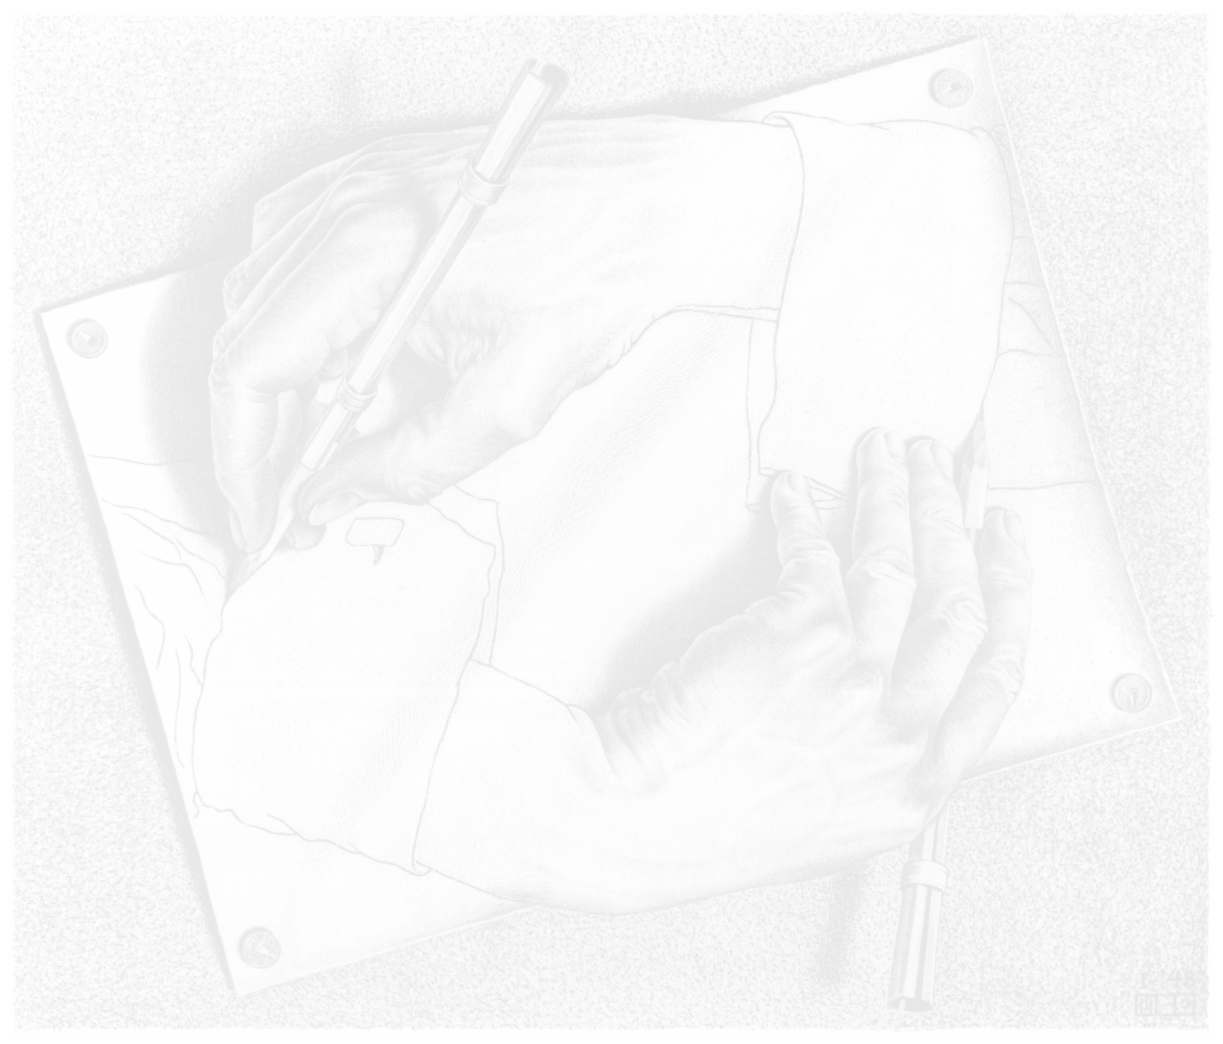
\includegraphics[width=\paperwidth, height=\paperheight]{./figure/theme/escher_hands_tr.png}
%    }
}

%\usetheme{Hannover}
\usetheme{Copenhagen}
\usecolortheme{seahorse}
\usecolortheme{rose}
%\usetheme{Frankfurt}
%\usecolortheme{beetle}

%\useoutertheme[subsection=false]{smoothbars}
%\useoutertheme[subsection=false]{smoothtree}
\useoutertheme{shadow}
\setbeamercovered{dynamic}

\pgfdeclareimage[height=1cm]{logo}{figure/theme/logo}
\logo{\pgfuseimage{logo}}

%New color
\definecolor{color1}{RGB}{184,184,228}
\definecolor{color2}{RGB}{214,214,240}
\definecolor{glicine}{RGB}{201, 160, 220}
\definecolor{darkorange}{RGB}{226,098,000}
\definecolor{emerald}{RGB}{000,128,000}
\definecolor{stroll}{RGB}{255,255,194}
\definecolor{newred}{RGB}{225,000,000}
\begin{document}

%%%%%%%%%%%%%%%%%%%%%%%%%%%%%%%%%%%%%%%%%%%%%%%%%%%%%

\begin{frame}
\maketitle
\end{frame}

%%%%%%%%%%%%%%%%%%%%%%%%%%%%%%%%%%%%%%%%%%%%%%%%%%%%%

\begin{frame}
\frametitle{Outline}
	\begin{multicols}{2}
		\tableofcontents
	\end{multicols}
\end{frame}

%%%%%%%%%%%%%%%%%%%%%%%%%%%%%%%%%%%%%%%%%%%%%%%%%%%%%

\begin{frame}
	\frametitle{mRMR in azione}
	\begin{tikzpicture}[scale=.8]
	\tikzstyle{every node} = [rectangle, fill=stroll, align=center, font=\scriptsize, draw=black, ultra thin]
	\node (input_data) at (0,0) {Input\\Data};
	\node (train_data) at (1,1.5) {Training\\Data};
	\node (test_data) at (1,-1.5) {Test\\Data};
	\node[fill=yellow] (feat_sel) at (3.5,1.5) {Feature\\Selection};
	\node[fill=newred, text=white] (mRMR) at (3.5,3) {mRMR};
	\node (red_data) at (6,1.5) {Reduced\\Data};
	\node (red_test_data) at (6,-1.5) {Reduced\\Test Data};
	\node (class) at (8.5,1.5) {Classifier};
	\node (rule) at (11,1.5) {Rule};
	\node (pred) at (11,-1.5) {Prediction};
	\node (class_label) at (11,-2.8) {Class Label};
	
	%Overlapping node to enhance the mRMR node
	\node[fill=none, draw=red, very thick, solid, fit=(mRMR), inner sep=0.2ex, ellipse] (over) {};
	\draw
	(input_data.5) -- ++(0.43,0) edge[->] (train_data)
	(input_data.0.5) -- ++(0.43,0) edge[->] (test_data)
	(train_data) edge[->] (feat_sel)
	(mRMR) edge[->] (feat_sel)
	(4.75,1.5) edge[->] (4.75,-1.5)
	(feat_sel) edge[->] (red_data)
	(test_data) edge[->] (red_test_data)
	(red_data) edge[->] (class)
	(class) edge[->] (rule)
	(red_test_data) edge[->] (pred)
	(pred) edge[->] (class_label)
	(rule) edge[->] (pred)
	;
	\end{tikzpicture}
\end{frame}

\section{Mutual Information}
\subsection{Definizione}
\begin{frame}
	\frametitle{Mutual Information - Definizione}
		\nocite{Ding:2003:MRF:937976.938050}
		\nocite{Peng05featureselection}
Date due variabili casuali \emph{X} e \emph{Y} con distribuzione di probabilità congiunta $p(x, y)$, la mutua
informazione è definita come \\~$$I(X; Y ) = H(X) − H(X|Y ) = H(Y ) − H(Y |X)$$\\~\\
La mutua informazione rappresenta i bit di informazione che una delle variabili fornisce circa l'altra
\begin{figure}[htb]
	\vspace{-0.2cm}
	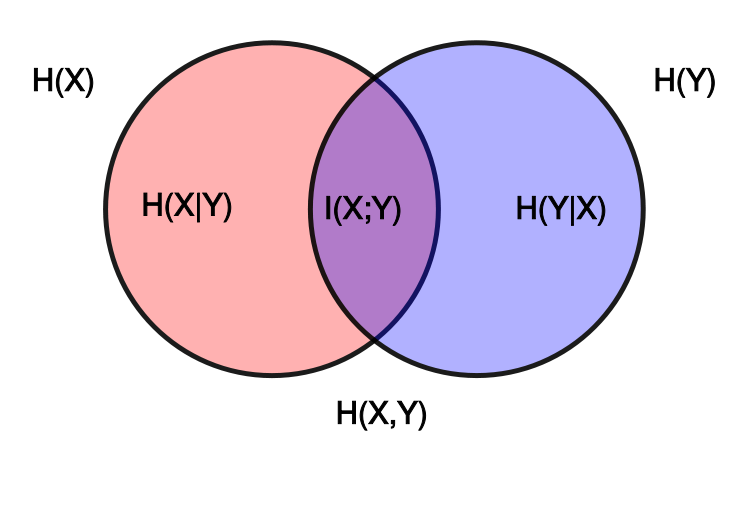
\includegraphics[width=0.48\textwidth]{figure/mutual.png}
\end{figure}
\end{frame}
\begin{frame}
	\frametitle{Considerazioni}
	\begin{itemize}
		\item $I(X;Y)=0 \Rightarrow$ \emph{X} e \emph{Y} sono variabili indipendenti
		\item $\pmb{I(X;Y)} = H(X)-H(X|Y)=H(Y)-H(Y|X)= \pmb{I(Y;X)}$
		\item $I(X;X)=H(X)$
	\end{itemize}
\end{frame}
\begin{frame}
	\frametitle{Esempio}
	Lanciamo 10 monete:
	\begin{itemize}
		\item \emph{X} rappresenta i valori delle prime 7 monete
		\item Y quelli delle ultime 5
	\end{itemize}
	Avremo che:
	\begin{columns}
		\begin{column}{0.5\textwidth}
			\begin{itemize}
				\item $H(X) = 7$
				\item $H(Y) = 5$\newline
			\end{itemize}
		\end{column}
		\begin{column}{0.5\textwidth}
			\begin{itemize}
				\item $H(X|Y) = 5$
				\item $H(Y|X) = 3$\newline
			\end{itemize}
		\end{column}
	\end{columns}
	La mutua informazione sarà quindi pari a
$$I(X; Y ) = I(Y ; X) = 2 $$
\end{frame}
\subsection{Formule}
\begin{frame}
	\frametitle{In caso di varibili discrete\dots}
	Definite due variabili casuali discrete \emph{X} e \emph{Y}
	$$ I (x;y) = \sum\limits_{y \in Y} \sum\limits_{x \in X} p(x,y)\log \frac{p(x,y)}{p(x)p(y)}$$
	dove
	\begin{itemize}
		\item $p(x,y)$ è la funzione di distribuzione di probabilità congiunta di \emph{X} e \emph{Y}
		\item $p(x)$ e $p(y)$ sono le funzioni di distribuzione di probabilità marginale di X e Y
	\end{itemize}
\end{frame}
\begin{frame}
	\frametitle{\dots mentre nel caso di variabili continue}
	$$ I (x;y) = \int_Y \int_X p(x,y)\log \frac{p(x,y)}{p(x)p(y)} \mathrm{d}x \mathrm{d}y$$
	dove
	\begin{itemize}
		\item $p(x,y)$ è la funzione di densità di probabilità congiunta di \emph{X} e \emph{Y}
		\item $p(x)$ e $p(y)$ sono le funzioni di densità di probabilità marginale di X e Y
	\end{itemize}
\end{frame}
\subsection{Problematiche}
\begin{frame}
	\frametitle{Problematiche}
	\begin{itemize}
		\item In caso di variabili continue, difficoltà nella computazione degli integrali nello spazio continuo su un numero limitato di campioni
	\end{itemize}
	\textbf{Soluzione}
	\begin{itemize}
		\item Incorporare la discretizzazione dei dati nella fase di preprocessing
	\end{itemize}
\end{frame}

%%%%%%%%%%%%%%%%%%%%%%%%%%%%%%%%%%%%%%%%%%%%%%%%%%%%%

\section{Max Dependency}
\subsection{Definizione}
\begin{frame}
	\frametitle{Max Dependency \dots}
	In termini di mutua informazione, l'obiettivo è trovare il set di feature \emph{S} con \emph{m} features che hanno la più alta dipendenza con la classe target \emph{c}
	$$ \max Dep(S,c)~~~~~ Dep = I(\{x_1,\dots,x_m \};c )$$
	Dove 
	\begin{itemize}
		\item $x_1,\dots,x_m$ sono le $m$ features selezionate
		\item $I$ indica la mutua informazione tra le feature del set
	\end{itemize}
\end{frame}

\subsection{Formula}
\begin{frame}
	\frametitle{\dots Max Dependency}
	\begin{itemize}
		\item Dato un set contenente \emph{m-1} features( $S_{m-1}$) l'\emph{m-}sima feature consiste  nella feature che più riesce ad incrementare la mutua informazione $I(S,c)$
	\end{itemize}
	
	\begin{align*}
	\hspace*{-0.6cm}
	I (S_m;c) &= \int\int p(S_m,c)\log \frac{p(S_m,c)}{p(S_m)p(c)} \mathrm{d}S_m \mathrm{d}c \\
	&= \int\int p(S_{m-1},x_m,c)\log \frac{p(S_{m-1},x_m,c)}{p(S{m-1},x_m)p(c)} \mathrm{d}S_{m-1}\mathrm{d}S_m\mathrm{d}c \\
	&=\int\dots\int p(x_1,\dots,x_m,c)\log \frac{p(x_1,\dots,x_m,c)}{p(x_1,\dots,x_m)p(c)} \mathrm{d}x_1,\dots,\mathrm{d}x_m \mathrm{d}c \\\\
	\end{align*}

\end{frame}

\subsection{Problemi}
\begin{frame}
	\frametitle{Problemi nel continuo}
	Difficoltà nella stima accurata delle funzioni di densità multivariate $p(x_1,\dots,x_m)$ e $p(x_1,\dots,x_m,c)$
	\begin{itemize}
		\item Numero di campioni insufficienti
		\item Comporta il calcolo delle inverse delle matrice di covarianza multidimensionali
		\item Computazione molto lenta
	\end{itemize}
\end{frame}

\begin{frame}
	\frametitle{Problemi nel discreto}
	Difficoltà nel calcolo delle funzioni di distribuzione di probabilità congiunta $p(x_1,\dots,x_m)$ e $p(x_1,\dots,x_m,c)$
	\begin{itemize}
		\item Numero di campioni insufficienti
		\item Computazione molto lenta in caso di un valore \emph{m} molto alto
	\end{itemize}
\end{frame}

\begin{frame}
	\frametitle{Soluzione}
	\begin{itemize}
		\item Approssimare la funzione di dipendenza ad una funzione computazionalmente meno onerosa
	\end{itemize}
	\begin{align*}
	Dependency &\approx Relevance ~ + ~ Redundancy ~~ \vee \\
	Dependency &\approx \frac{Relevance}{Redundancy}
	\end{align*}
\end{frame}

%%%%%%%%%%%%%%%%%%%%%%%%%%%%%%%%%%%%%%%%%%%%%%%%%%%%%

\section{Max Relevance}
\subsection{Definizione}
\begin{frame}
	\frametitle{Max Relevance - Definizione}
	\begin{itemize}
		\item Ricercare le feature che riescano ad approssimare la funzione 	$$ \max Dep(S,c)~~~~~ Dep = I(\{x_1,\dots,x_m \};c )$$
		con il valor medio di tutti i valori della mutua informazione tra le singole feature $x_i$ e la classe $c$
	\end{itemize}
\end{frame}
\subsection{Formule}
\begin{frame}
	\frametitle{Per variabili discrete}
	In caso di variabili discrete l'obiettivo sarà massimizzare la funzione \emph{Dep} calcolata nel seguente modo
	$$Dep(S,c)= \frac{1}{|S|} \sum\limits_{x_i \in S} I (x_i;c)$$
	dove 
	\begin{itemize}
		\item S indica il set contenente tutte le features
		\item $x_i$ indica la \emph{i-}sima feature da considerare
		\item $c$ indica la classe target
	\end{itemize}
\end{frame}

\begin{frame}
	\frametitle{Per variabili continue\dots}
	Per le variabili continue bisogna usare la \emph{F-}statistic come misura per calcolare la rilevanza tra le features $x_i$ e la classe target \emph{c}
	$$ F(x_i,c) = \frac{\frac{\sum\limits_{K}{n_k(\bar{x_k}-\bar{x})}}{K-1}}{\sigma^2}$$
	dove: 
	\begin{itemize}
		\item $\sigma^2=\frac{ \sum\limits_{k}{(n_k-1)\sigma^2_k}}{n-K}$
		\item $k$ indica le classi denotate da $c$
		\item $\bar{x}$ è il valor medio di $x_i$ di tutti i campioni
		\item $\bar{x_k}$ è il valor medio di $x_i$ di tutti i campioni di classe $k$
		\item $n_k$ e $\sigma_k$ indicano dimensione e varianza della $k-$classe
	\end{itemize}
\end{frame}

\begin{frame}
	\frametitle{\dots per variabili continue}
	In caso di variabili continue l'obiettivo sarà massimizzare la funzione \emph{Dep} calcolata nel seguente modo
	$$Dep(S,c)= \frac{1}{|S|} \sum\limits_{x_i \in S} F(x_i;c)$$
	dove 
	\begin{itemize}
		\item $F$ indica la funzione $F-test$ calcolata sulle feature in relazione alla classe target
		\item $S$ indica il set contenente tutte le features
		\item $x_i$ indica la \emph{i-}sima feature da considerare
		\item $c$ indica la classe target
	\end{itemize}
\end{frame}

\subsection{Problematiche}
\begin{frame}
	\frametitle{Problematiche}
	\begin{itemize}
		\item Features selezionate in questo modo potrebbero essere ricche di \textbf{ridondanza}\newline
		\item Se due features dipendono l'una dall'altra è probabile che eliminando una di esse il potere discriminante non sarà decrementato
	\end{itemize}
\end{frame}

%%%%%%%%%%%%%%%%%%%%%%%%%%%%%%%%%%%%%%%%%%%%%%%%%%%%%
\section{Min Redundancy}
\subsection{Definizione}
\begin{frame}
	\frametitle{Min Redundancy - Definizione}
	\begin{itemize}
		\item Consiste nel selezionare le features in modo tale che siano tra loro più dissimilari possibili
		\item Il subset che si otterrà sarà il più rappresentativo possibile dell'intero dataset
	\end{itemize}
	Formalmente consiste nel 
	\begin{itemize}
	\item Calcolare una funzione \textbf{Red} calcolata sul set di feature $S$
	\item Trovare il subset che minimizza la funzione calcolata
	\end{itemize}
	$$\min Red(S)$$
\end{frame}

\subsection{Formule}
\begin{frame}
	\frametitle{Per variabili discrete}
	$$Red (S)= \frac{1}{|S|^2} \sum\limits_{x_i,x_j \in S} I (x_i;x_j)$$
	dove 
	\begin{itemize}
		\item $|S|(= m)$ è il numero di features presenti nel subset $S$
		\item $x_i$ e $x_j$ rappresentano rispettivamente la $i$-esima e $j$-esima feature del subset $S$
		\item $I (x_i;x_j)$ rappresenta la mutua informazione tra le due feature
	\end{itemize}
\end{frame}

\begin{frame}
	\frametitle{Per variabili continue}
	$$Red(S)= \frac{1}{|S|^2} \sum\limits_{x_i,x_j \in S} |c (x_i;x_j)|$$
	dove 
	\begin{itemize}
		\item $|S|(= m)$ è il numero di features presenti nel subset $S$
		\item $x_i$ e $x_j$ rappresentano rispettivamente la $i$-esima e $j$-esima feature del subset $S$
		\item $|c (x_i;x_j)|$ indica il valore assoluto del coefficiente di correlazione di Pearson tra le feature $x_i$ e $x_j$
	\end{itemize}
\end{frame}

%%%%%%%%%%%%%%%%%%%%%%%%%%%%%%%%%%%%%%%%%%%%%%%%%%%%%

\section{mRMR}
\subsection{Definizione}
\begin{frame}
	\frametitle{mRMR - Definizione}
	Approccio basato sulla combinazione della
	\begin{itemize}
		\item \textbf{minima ridondanza} tra le features
		\item \textbf{massima rilevanza} delle features con la classe target
	\end{itemize}
\end{frame}

\subsection{Formule}
\begin{frame}
	\frametitle{Calcolo mRMR}
	\begin{itemize}
		\item Variabili discrete
			\begin{itemize}
				\item MID - Mutual information difference
				\item MIQ - Mutual information quotient\newline
			\end{itemize}
		\item Variabili continue
			\begin{itemize}
				\item FCD - F-test correlation difference
				\item FCQ - F-test correlation quotient
			\end{itemize}
	\end{itemize}
\end{frame}
\begin{frame}
	\frametitle{Discrete - MID}
	Consiste nel trovare le features che massimizzino la differenza tra dipendenze e ridondanze di queste features dalla classe target attraverso il calcolo della mutua informazione
	$$\max (Dep(S,c) - Red(S))$$
	dove ricordiamo che
	\begin{itemize}
		\item $Dep(S,c)= \frac{1}{|S|} \sum\limits_{x_i \in S} I (x_i;c)$
		\item $Red (S)= \frac{1}{|S|^2} \sum\limits_{x_i,x_j \in S} I (x_i;x_j)$
	\end{itemize}
\end{frame}

\begin{frame}
	\frametitle{Discrete - MIQ}
	Consiste nel trovare le features che massimizzino il rapporto tra dipendenze e ridondanze di queste features dalla classe target attraverso il calcolo della mutua informazione
	$$\max\frac{Dep(S,c)}{Red(S)}$$
	dove ricordiamo che
	\begin{itemize}
		\item $Dep(S,c)= \frac{1}{|S|} \sum\limits_{x_i \in S} I (x_i;c)$
		\item $Red (S)= \frac{1}{|S|^2} \sum\limits_{x_i,x_j \in S} I (x_i;x_j)$
	\end{itemize}
\end{frame}
\begin{frame}
	\frametitle{Continuous - FCD}
	Consiste nel trovare le features che massimizzino la differenza tra dipendenze e ridondanze di queste features dalla classe target attraverso il calcolo del F-test
	$$\max((Dep(S,c) - Red(S))$$
	dove ricordiamo che
	\begin{itemize}
		\item $Dep(S,c)= \frac{1}{|S|} \sum\limits_{x_i \in S} F(x_i;c)$
		\item $Red(S)= \frac{1}{|S|^2} \sum\limits_{x_i,x_j \in S} |c (x_i;x_j)|$
	\end{itemize}
\end{frame}

\begin{frame}
	\frametitle{Continuous - FCQ}
	Consiste nel trovare le features che massimizzino il rapporto tra dipendenze e ridondanze di queste features dalla classe target attraverso il calcolo del F-test
	$$\max\frac{Dep(S,c)}{Red(S)}$$
	dove ricordiamo che
	\begin{itemize}
		\item $Dep(S,c)= \frac{1}{|S|} \sum\limits_{x_i \in S} F(x_i;c)$
		\item $Red(S)= \frac{1}{|S|^2} \sum\limits_{x_i,x_j \in S} |c (x_i;x_j)|$
	\end{itemize}
\end{frame}

\subsection{Benefici}
\begin{frame}
	\frametitle{Benefici}
	\begin{itemize}
		\item Con lo stesso numero di features, mRMR garantisce maggiore rappresentatività al dataset offrendo una migliore proprietà di generalizzazione
		\item Allo stesso modo, possiamo usare un set di feature mRMR più piccolo per ricoprire in maniera più efficace lo stesso spazio ricoperto da feature set convenzionale più grande
	\end{itemize}
\end{frame}
%%%%%%%%%%%%%%%%%%%%%%%%%%%%%%%%%%%%%%%%%%%%%%%%%%%%%

\section{Algoritmo}
\begin{frame}
	\frametitle{Feature Selection}
	La fase di Feature Selection avverrà in modalità \textbf{two stage}:
	\begin{enumerate}
		\item Selezione del candidate feature set tramite l'utilizzo della tecnica mRMR
		\item Utilizzo del wrapper model per una ulteriore selezione di feature partendo dal candidate feature set
	\end{enumerate}
	\begin{figure}[htb]
		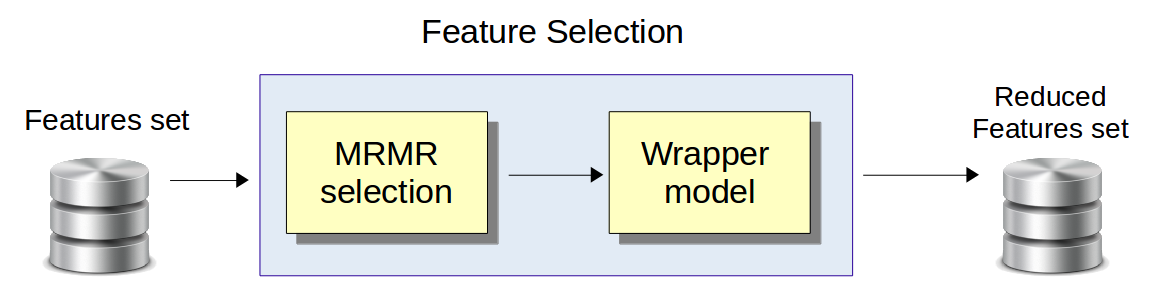
\includegraphics[width=.9\textwidth]{figure/twostage.png}
	\end{figure}
\end{frame}
\begin{frame}
	\frametitle{Fase 1 - Selezione del Candidate Feature Set}
	\begin{enumerate}
		\item Vengono creati $n$ subset sequenziali di feature tramite la selezione incrementale mRMR nella forma
		$$S_1 \subset S_2 \subset \dots \subset S_{n-1} \subset S_n $$
		\item Per ogni subset $S_k$ con $1 \leq k \leq n$, verrà calcolato l'errore di cross-validation $e_k$ ed inserito in un insieme $\Omega$.
		\item Viene selezionato il subset $S_{n^*}$ dove $n^*$ è il subset avente come errore $e^*$ il più piccolo errore di cross validation $\in \Omega$.
	\end{enumerate}
\end{frame}

\begin{frame}
	\frametitle{Fase 2 - Wrapper Model}
	\begin{itemize}
		\item Il subset candidato sarà il subset dato in input al wrapper
		\item Utilizzo di 4 tecniche di feature selection
			\begin{itemize}
				\item Na\"ive Bayes (NB) classifier
				\item Support Vector Machine (SVM)
				\item Linear Discriminant Analysis (LDA)
				\item Logistic Regression (LR)
			\end{itemize}
		\end{itemize}
\begin{figure}[htb]
	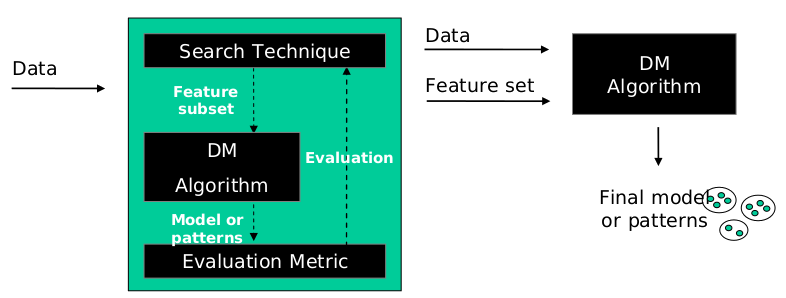
\includegraphics[width=.70\textwidth]{figure/wrapper.png}
\end{figure}
\end{frame}

\begin{frame}
	\frametitle{Na\"ive Bayes (NB) classifier}
	\begin{itemize}
		\item Si basa sul \textbf{Teorema di Bayes}
		\item Tutte le feature sono indipendenti tra loro (\textbf{indipendence assumption})
	\end{itemize}
	$$p(h_k|s) \propto \prod_{i \in S}{p(g_i|h_k)}$$ dove 
	\begin{itemize}
		\item $s$ = Set di $m$ feature cosi composto $s= \{ g_1,g_2,\dots,g_m \}$
		\item $p(h_k|s)$ = probabilità a posteriori che un set $s$ appartenga alla classe $h_k$
		\item $ p(g_i|h_k)$ = probabilità a posteriori che la feature $g_i$ sia di classe $h_k$
	\end{itemize}
\end{frame}

\begin{frame}
	\frametitle{Support Vector Machine (SVM)}
	\begin{itemize}
		\item SVM massimizza il \emph{margine} di separazione tra gli iperpiani
		\item La funzione di decisione viene creata sulla base del subset di esempi (\emph{support vectors})
	\end{itemize}
	\begin{figure}[htb]
		\vspace{-0.2cm}
		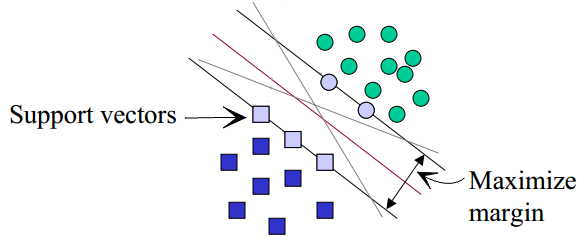
\includegraphics[width=.80\textwidth]{figure/svm.png}
	\end{figure}
\end{frame}

\begin{frame}
	\frametitle{Linear Discriminant Analysis (LDA)}
	Metodo di classificazione che sfrutta la combinazione lineare tra feature sotto determinate assunzioni:
	\begin{columns}[c]
		\begin{column}{.5\textwidth}
			\begin{figure}[htb]
				\vspace{-0.2cm}
				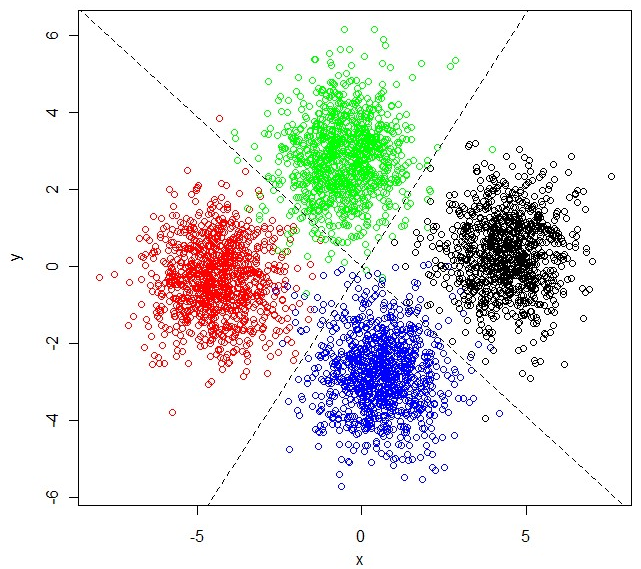
\includegraphics[width=1\textwidth]{figure/LDA.png}
			\end{figure}
		\end{column}
		\begin{column}{.5\textwidth}
			\begin{itemize}
				\item Ogni campione segue una distribuzione Gaussiana
				\item Nessuna correlazione tra feature
			\end{itemize}
		\end{column}
	\end{columns}
\end{frame}

\begin{frame}
	\frametitle{Logistic Regression (LR)}
	\begin{itemize}
		\item Caso particolare di modello lineare generalizzato
		\item Applicazione di una funzione logistica alla combinazione lineare delle feature in modo da limitarla in un intervallo $[0;1]$ 
%		$$F(x)=\frac{1}{1+e^{-(\beta_0+\beta_1x)}}$$
	\end{itemize}
	\begin{figure}[htb]
		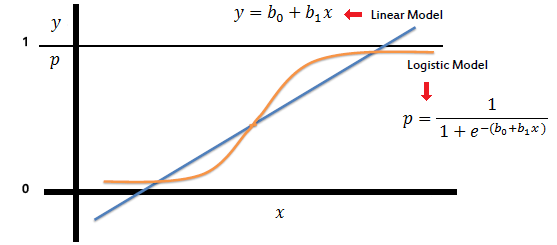
\includegraphics[width=.9\textwidth]{figure/LogReg.png}
	\end{figure}
\end{frame}

%%%%%%%%%%%%%%%%%%%%%%%%%%%%%%%%%%%%%%%%%%%%%%%%%%%%%
\section{Sperimentazione}
\begin{frame}
	\frametitle{Sperimentazione \dots}
	La sperimentazione eseguita aveva i seguenti parametri:
	\begin{itemize}
		\item Esecuzione su 6 dataset di geni contenenti sia attributi discreti che continui
		\item Goal: Verificare se l'approccio mRMR potesse migliorare le performance di classificazione
		\item Configurazioni
		\begin{itemize}
			\item Baseline + wrapper (NB, SVM, LDA, LR)
			\item mRMR approach + wrapper (NB, SVM, LDA, LR)
		\end{itemize}
	\end{itemize}
\end{frame}

\begin{frame}
	\frametitle{\dots Sperimentazione}
	I risultati mostrano che mRMR performa meglio della baseline su tutte le configurazioni, in particolare
	\begin{itemize}
		\item Su variabili discrete la scelta migliore ricade su MIQ
		\item Su variabili continue la scelta migliore ricade su FCQ
		\item Framework mRMR indipendente dal metodo predittivo utilizzato
		\item mRMR riesce con meno feature della baseline ad eguagliare e migliorare le performance
	\end{itemize}
\end{frame}

\begin{frame}{Bibliography}
	\frametitle{References}
	\bibliographystyle{alpha}
	\bibliography{mybib}
\end{frame}
\end{document}
